\chapter{Aufgabe 4}
\section{Repo zur Aufgabe 4}
In diesem Repo auf Gitlab befindet sich die Bearbeitung des Programmierteils der Aufgabe 4. 
In dieser Aufgabe soll ein C-Programm geschrieben werden dass ein Datum eingegen nimmt und den entsprechenden Wochentag berechnet.
Das Programm soll für verschiedene Definitionsbereiche angepasst werden. \par
\href{https://gitlab.thga.de/daniel.krueger/pruefung_sose_2023_aufgabe_4_getopt}{\textbf{LINK}}

\section{Erweiterung des Programms}
Die Programme die sich in dem Repo befinden, wurden mithilfe des Algorithmus von Christian Zeller geschrieben.
Um diesen nutzen zu können, müssen die Monate in Julianischer Zählung angegeben werden.
Dies liegt daran das der uns bekannte gregorianische Kalender erst 1582 beginnt und somit keine Daten davor anbietet.
Dabei wird die Reihenfolge so verschoben, dass der Februar am Ende des Jahres steht.
Dies muss geschehen da der Februar ein Schaltmonat ist und somit mit seiner Unregelmäßigkeit am Ende des Jahres steht.
Der Februar hat damit keinen Einfluss auf die darauf folgenden Monate des Jahres.
Das Jahr geht demnach von März bis Februar.\par
Mit dieser Anpassung der Monate und dem Algorithmus von Zeller können die Wochentage beginnend vom 0000-01-01 berechnet werden.\par
In meinem speziellen Fall sind alle Programme bereits mit dem Algorithmus geschrieben worden.
Lediglich die if-Abfrage, wie in Abbildung \ref{definitionsbereich} zu sehen ist, begrenzt den Definitionsbereich.

\begin{figure}[h]
	\centering
	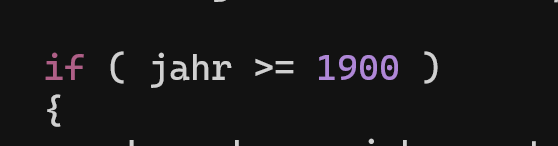
\includegraphics[scale=0.7]{Images/Definitionsbereich_4.png}
	\caption{Begrenzung des Definitionsbereichs der Datums Eingabe}
	\label{definitionsbereich}
\end{figure}

Es müsste lediglich diese Abfrage entfernt werden, wie es in dem Beispiel Programm main\_3.c in dem Repo erfolgt ist. 
Alternativ, um sicherzustellen das nur Daten ab dem Jahr nur 0 eingegeben werden können, müsste in der if-Bedingung vorausgesetzt werden dass das Jahr größer gleich Null ist.
\begin{lstlisting}
if ( jahr >= 0 ]
{
\end{lstlisting}
